\scanpage{131}
\mspage{64}

On constate que les composés
\[
T_\pi \xrightarrow{\sim} L_i \longrightarrow
H^2(\pi,\widehat{\mathbb Z})^{\unsure{\otimes-1|\theta-1}}
\]
ne dépendent pas du choix de $i$, de sorte que le module d'orientation $T_\pi$ du groupe \inserted{profini $\pi$} \unsure{à lacets} $\pi$ s'identifie au \uline{dual} de $H^2(\pi,\widehat{\mathbb Z})$ (si $g\ne0$).

Considérons maintenant un hom. de groupes à lacets
\[
\begin{gathered}
\pi'\xrightarrow{f}\pi\\
I'_0\xrightarrow{\tau}I
\end{gathered}
\]
associé à un isom $T_{\pi'}\simeq T_\pi$ et une application degré
$d:I'_0\longrightarrow\mathbb N$
\deleted{(\unsure{entiers} \illegible{3}}
(NB $i'\in I'\setminus I'_0\longrightarrow f(L'_{i'})=(1)$).

On \unsure{voudrait} en déduire un diagramme de morphismes de topos
\diagram{\begin{tikzcd}[ampersand replacement=\&]
B_{\unsure{\Pi_1 U'}} \arrow[r] \arrow[d] \& B_{\deleted{\unsure{\Pi_1}}X',U'} \arrow[r] \arrow[d] \& B_{\unsure{\Pi_1 X'}} \arrow[d] \\
B_{\unsure{\Pi_1 U}} \arrow[r] \& B_{\deleted{\unsure{\Pi_1}}X,U} \arrow[r] \& B_{\unsure{\Pi_1 X}}
\end{tikzcd}}
et un hom \uline{\unsure{trace}} sur la cohomologie à supports propres de $U',U$ (définie en termes de cohomologie sur $B_{X',U'}, B_{X,U}$ relativement)
\deleted{\unsure{qui un iso}} \unsure{induisant} \deleted{\unsure{pour}} un \uline{iso}
\[
\unsure{H^2_!}(U',\widehat{\mathbb Z})\longrightarrow
\unsure{H^2_!}(U,\widehat{\mathbb Z})
\]

\scanpage{132}

qui soit justement \inserted{(contragrédient de)} (l'isom des modules d'orientation associé à $f$....

14. Où on \unsure{revient} sur les morphismes \inserted{\unsure{non}} \uline{stricts} \unsure{correspondants}, dans le cadre topologique, au cas de
$f:(X',S')\longrightarrow(X,S)$ tels que l'on ait
$[f(X'\setminus S')\subset X\setminus S$, i.e.\ \inserted{$S'\supset f^{-1}(S)$,} \inserted{mais}$]$
\deleted{\illegible{1}} $S'\ne f^{-1}(S)$, i.e.\ il y a des pts de $\unsure{S'|S}$ qui sont envoyés dans $U=X\setminus S$.
\margin{$X,X'$ \unsure{$T$-orientés|$\Gamma$-orientés}}

Dans le \deleted{langage} \inserted{\unsure{prolangage|prolongement}} \unsure{toposique} et groupoïdal, $(X,S)$ est \deleted{défini} \inserted{décrit} par un diagramme de groupoïdes
\[
\unsure{\Pi_{D^*}|\Pi_1 D^*}\longrightarrow\unsure{\Pi_U|\Pi_1 U}
\qquad
(\text{et }k:T_{\unsure{\Pi_{D^*}}}\simeq
\text{ système local des }\pi_1\text{ sur }\unsure{\Pi_{D^*}})
\]
\deleted{\illegible{1}}
ou de topos
\[
B_{D^*}\longrightarrow B_U
\]
et \deleted{\unsure{un}} isom \inserted{$k$} du syst. local des $\pi_1$ sur $B_{D^*}$, \unsure{au} système \deleted{\unsure{constant}} \inserted{\unsure{const.}} $T$;
\deleted{\illegible{4} $(\deleted{\unsure{X}},U')$}
\inserted{qui permet de définir $B_D\;(=B_{\unsure{\pi_0 D_*}})$ (le topos discret)}
et le topos $B_{X,U}$, s'insérant dans le diagramme \deleted{$\unsure{B_{\Pi_1 D^*}}$} de topos

\scanpage{133}
\mspage{65}

\diagram{\begin{tikzcd}[ampersand replacement=\&,column sep=large]
\& B_{D^*}\arrow[dl,"\rho"']\arrow[dr,"\sigma"] \& \\
B_U\arrow[dr,"\varphi"'] \&\& B_D\; (\text{topos discret }\simeq B_S)\arrow[dl,"\psi"] \\
\& B_{X,U} \&
\end{tikzcd}}
où $\varphi,\psi$ sont des morphismes d'inclusion de sous-topos, $\varphi$ ouvert $\psi$ fermé, complémentaires l'un de l'autre, et idem pour $(X',S')$, décrit par un diagramme analogue
\diagram{\begin{tikzcd}[ampersand replacement=\&]
\& B_{D'^*}\arrow[dl]\arrow[dr] \& \\
B_{U'}\arrow[dr] \&\& B_{D'}\simeq\unsure{B_{S'}|B_S}\arrow[dl] \\
\& B_{X',U'} \&
\end{tikzcd}}

Ceci dit, on veut absolument, dans une description de
$f:(X',S')\longrightarrow(X,S)$, que celle-ci permette de retrouver non seulement $B_{U'}\longrightarrow B_U$ (ce qui sera acquis par la donnée d'un $f_\pi:\pi'\longrightarrow\pi$), mais aussi
\[
B_{X',U'}\longrightarrow B_{X,U}\qquad\unsure{g|q}.
\]
On a \deleted{\unsure{$S$}}
\[
S'=\underset{\substack{\Vert\\f^{-1}(S)}}{S'_0}\amalg S'_1,
\quad\text{et}\quad D'=D'_0\amalg D'_1
\]

\scanpage{134}
\mspage{66}

et en fait $f$ induit $S'_1\xrightarrow{f}U$ (et non $S'_1\longrightarrow S$) qui doit s'expliciter, au niveau \deleted{\illegible{2}} des topos multigaloisiens, par un morphisme
\diagram{\begin{tikzcd}[ampersand replacement=\&]
B_{D'_1}\arrow[r] \& B_U \\
B_{S'_1}\arrow[u,"\simeq",draw=none] \&
\end{tikzcd}}
i.e.\ par la donnée d'une famille de rev. universels de $U$, paramétrée par $S'_1=I'_1$, ou (\unsure{si un tel} rev. universel est choisi, $U$ étant connexe, d'où un $\pi=\operatorname{Aut}(\widetilde U)$) par une famille de torseurs sous \deleted{\unsure{le}} $\pi$, $(P_{i'})_{i'\in I'_1}$.
Ceci étant \deleted{\unsure{défini}} \inserted{posé} on \unsure{pourra} décrire, en termes de
\diagram{\begin{tikzcd}[ampersand replacement=\&,column sep=3.5em,row sep=3em]
B_{D_0'{}^*} \arrow[r,no head] \arrow[d] \& B_{U'} \arrow[d] \\
B_{D^*} \arrow[r,no head]
\arrow[ur,bend left=30,shorten <=1.5em,shorten >=1.5em,"\sim"'] \& B_U
\end{tikzcd}}
et de
\[
B_{D_1'^*}\longrightarrow B_{D'_1}\longrightarrow B_U
\]
\deleted{\unsure{un}} \inserted{\unsure{un}} hom de topos $B_{X',U'}\longrightarrow B_{X,U}$
--- je passe sur le détail de la description
\margin{Il \unsure{semble} qu'on soit en droit de faire la \unsure{description} des morphismes de topos $B_{X',U'}\longrightarrow B_{X,U}$ qui induisent $U'\longrightarrow U$ et qui sur $D_1'^*$ \deleted{\illegible{3}}, se factorisent par $D_1'^*\longrightarrow D'_1$...}

\scanpage{135}

Quand on se donne un groupe d'opérateurs $\unsure{\Gamma}$ sur la situation $(X',S')\longrightarrow(X,S)$ donc sur la situation groupoïdale ou \unsure{topossique|toposique}, il faut en tenir compte dans la description ci-dessus.
Ainsi $I'_0$ et $I'_1$ sont stables par $\Gamma$, et le morphisme \deleted{\illegible{1}} $B_{\unsure{D'_1}}\longrightarrow B_U$ doit être stable par $\Gamma$.
\deleted{On a donc un \unsure{joli} ensemble $\unsure{E_f=\bigcup E_i}$ ---}
\deleted{En termes d'un rev. universel $\widetilde U$ de $U$, considérons \unsure{l'ensemble des} $\unsure{\operatorname{Hom}}(f_*(\unsure{s'_{i'}}),\widetilde U)$}
Ce qui signifie aussi, sans doute, qu'on a un morphisme de topos de
$B_{D'_1,\unsure{\Sigma|\Gamma}}=B_{I'_1,\unsure{\Sigma|\Gamma}}$
dans $B_{U,\unsure{\Gamma}}$.
Choisissant pour tte orbite de $\Gamma$ dans $I'_1$ un représentant $s'\in I'_1$, et considérant son stabilisateur $\Gamma_{s'}\subset\Gamma$, il faut donc pour tte telle orbite i.e.\ \deleted{\unsure{tte}} \unsure{tel $s'$} \unsure{se} donner un $\Gamma_{s'}$ objet de la cat. des rev. universels de $(U,\Gamma)$.
\unsure{Équivalemment} \deleted{donc} \unsure{Décrivant} $(U,\Gamma)$ en termes

\scanpage{136}
\mspage{67}

d'une extension $\mathcal E$ de \deleted{\unsure{$\Sigma$}} $\Gamma$ par $\pi$ (en choisissant un rev. universel $\widetilde U$ de $U$), la donnée de $B_{\Gamma_{s'}}\longrightarrow B_{X,U}$ compatible avec tout revient \unsure{simplement} à : la donnée d'un torseur $P$ à droite sous $\pi$ (permettant de tordre le revêtement universel \illegible{1} $\widetilde U$ de $\unsure{U^\Gamma}$ à l'aide de $P$ \deleted{et} \inserted{donc aussi de tordre $\mathcal E$ par $P$}), et d'un scindage de $\mathcal E^P\longrightarrow\Gamma$ au dessus de $\Gamma_{s'}$.
[La classe d'isomorphie d'un tel objet $\longrightarrow$ une classe de $\pi$-conjugaison de scindages de $\mathcal E\longrightarrow\Gamma$ au dessus de $\Gamma_{s'}$... ).

Un autom d'un tel couple \deleted{correspond} $P,\ \Gamma_{s'}\xrightarrow{q}\mathcal E^P$ correspond à un $\alpha\in\pi$ qui \uline{centralise} $\Gamma_{s'}$, \inserted{i.e.\ qui est fixé par $\Gamma_{s'}$ opérant sur $\pi$.} (Si les $\Gamma_{s'}$ opèrent assez fortement sur $\pi$ pour que l'on sache que $\pi^{\Gamma_{s'}}=(1)$, l'objet $(P,q:\Gamma_{s'}\longrightarrow\mathcal E^P)$ est défini à \uline{isom unique} près par la classe d'isomorphie \deleted{\unsure{de celui-ci}} (classe de scindages de $\mathcal E$ sur $\Gamma_{s'}$).
\margin{\figure{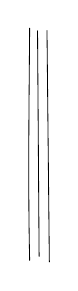
\begin{tikzpicture}[x=1cm,y=1cm,line cap=round]
\draw[line width=0.3pt] (0,0) .. controls (-0.01,-1.1) and (-0.02,-2.1) .. (0,-2.95);
\draw[line width=0.3pt] (0.10,-0.035) -- (0.12,-2.90);
\draw[line width=0.3pt] (0.22,-0.03) -- (0.25,-2.97);
\end{tikzpicture}}}
Il me semble probable que ceci soit tjrs le cas dans le cas \uline{arithmétique}, où $\Gamma_{s'}$ est un sr-groupe ouvert du groupe de Galois $\Gamma_k$ dont l'opération extérieure est \inserted{\unsure{dite canonique !}}).

\scanpage{137}

Ceci va en direction de la conjecture qu'une classe de scindage de $\mathcal E$ sur $\Gamma$ est ``aussi bonne'' qu'un pt rat. de $U$ sur $K$ --- et permet de \unsure{prodiguer} ce qu'un tel pt rationnel permettrait d'obtenir....

\textcircled{15} \uline{Retour sur le cas topologique} Soit $\Gamma$ un grpe fini opérant sur un grpe à lacets $\pi$ --- supposons que ceci provienne d'une situation topologique, $\Gamma$ opérant sur $(X,S)$. Il y a des pts à vérifier (\uline{cas anodins})
\margin{Structure des orbites critiques en termes d'extension...}

\[
\text{a) Opération de }\Gamma\text{ triviale}
\quad\Longleftrightarrow\quad
\Gamma\underset{\text{triviale}}{\longrightarrow}\operatorname{Autext}(\pi)
\]
en d'autres termes : un autom d'ordre fini de $(X,S)$ ne peut être isotope à l'identité (ou $\overline{\mathrm m}$ \inserted{seulement} homotope, cela revient au $\overline{\mathrm m}$ d'ailleurs) que si elle est triviale.

C'est $\unsure{\overline{\mathrm m}}$ \unsure{connu} en Géom. Alg ``abstraite'', du moment qu'on admet que $\unsure{U|u}$ possède une structure \deleted{\unsure{complexe}} \inserted{complexe}, \deleted{\unsure{conforme}} \inserted{\illegible{4}}

\scanpage{138}
\mspage{68}

\unsure{aussi bien|ainsi l'on} \deleted{suppose} \inserted{admet} qu'il n'y a pas de sauvagerie.... \unsure{Sans doute} tte action d'un groupe fini $\Gamma$ laisse structure conforme invariante, \deleted{\illegible{1}} donc sa restriction à
\[
\Gamma^0=\operatorname{Ker}(\Gamma\xrightarrow{\chi}\{\pm1\})
\]
laisse structure complexe invariante.

Supposons dorénavant que $\Gamma$ opère fidèlement, \inserted{$\Gamma\ne1$,} \deleted{\illegible{1}} Le choix d'une structure complexe sur $Y=X/\Gamma^0$ \inserted{en définit une sur $X$;} (NB: \deleted{\illegible{1}} $\Gamma/\Gamma^0$ opère encore \inserted{sur $X/\Gamma^0$} en fait \deleted{$X/\Gamma^0$} \unsure{si} $\Gamma\ne\Gamma^0$ i.e.\ $\Gamma/\Gamma^0\simeq\{\pm1\}$, $X/\Gamma^0$ est munie d'une ``structure de \deleted{\illegible{2}} courbe algébrique \inserted{str. conforme} réelle''... ) stable par $\Gamma^0$ --- et (stable par $\Gamma$ si on choisit celle de $Y$ \deleted{\unsure{invariante}} \inserted{invariante} par l'action \unsure{non triviale} de $\Gamma/\Gamma^0$ (s'il y en a).).
\margin{comme chaque fois \unsure{qu'on a un} rev. ramifié de surfaces conformes}

\deleted{Or} Tout $x\in U^\Gamma$ définit une classe \deleted{\illegible{1}} \inserted{\deleted{\unsure{classe}} de $\pi$-conj. de} scindages de l'extension $\mathcal E$ de $\Gamma$ par $\pi$, comme on voit en prenant $x$ comme pt base. ! Noter que $U^\Gamma$ est un ens fini \inserted{si $\Gamma^0\ne1$, [i.e.\ $\Gamma$ pas réduit à une \deleted{\illegible{1}} \illegible{3}]}.
\margin{\uline{NB} $U^\Gamma\ne\varnothing$ implique que $\unsure{\Gamma|\Gamma^0}$ est cyclique...}
On trouve \deleted{donc} une application
\[
U^\Gamma\longrightarrow\text{ens des classes de }\pi\text{-conjugaison de scindages de }\mathcal E\longrightarrow\Gamma,
\]

\scanpage{139}
\mspage{69}

i.e.\ \deleted{aux} des relèvements de $\Gamma\longrightarrow\operatorname{Autext}\pi$ \inserted{en} $\Gamma\longrightarrow\operatorname{Aut}(\pi)$, mod $\pi$-conjugaison.

\uline{Question} \inserted{(Si $\Gamma^0\ne(1)$)} Cette application est-elle bijective ??

[Si $\Gamma^0=\{1\}$, $\Gamma/\Gamma^0\simeq\{\pm1\}$, alors $X^\Gamma$ est l'ens des pts réels d'une courbe alg. réelle et $U^\Gamma=X^\Gamma-S^\Gamma$ est le complémentaire d'une partie finie dedans, on a
\[
\pi_0(X^\Gamma-S^\Gamma)\longrightarrow
\pi\text{-classes de scindages de }\mathcal E\text{ sur }\Gamma
\]
et la \deleted{\illegible{1}} question \uline{analogue} de bijectivité se pose, pour ext. de $\pm1$ par $\pi$... ]

Pour l'injectivité de l'application ds le cas $\Gamma^0\ne(1)$, \deleted{\unsure{Obs}} $\Gamma=\unsure{\Gamma^0_a|\Gamma^0}\simeq\mathbb Z/p\mathbb Z$, avec $p$ premier, i.e.\ $\Gamma$ engendré par un autom complexe $\unsure{\gamma}$ d'ordre $p$, qui définit (si $x,y\in U^\Gamma$, $\unsure{x\ne y}$) un autom d'ordre $p$ de $\pi_1(U,x)$, \unsure{soit} $u_x$ \unsure{soit} \deleted{une} classe dans les $\pi$-conj d'automs de $\pi$ d'ordre $p$), et un autre $u_y$.
Il faut prouver que $u_x,u_y$ ne sont pas conjugués sous $\pi$

\scanpage{140}

\uline{Théorème} Soit $\unsure{U|X}$ \deleted{\unsure{une surface}} \inserted{espace} topologique connexe \inserted{(\deleted{\illegible{2}}, par arcs)}, $\Gamma$ un groupe fini opérant \deleted{fidèlement} sur $U$, $\widetilde U$ un revêtement universel de $U$, d'où \deleted{opérant} un groupe extension
\[
1\longrightarrow\pi\xrightarrow{i}\mathcal E\xrightarrow{p}\Gamma\longrightarrow1
\]
agissant fidèlement sur $\widetilde U$ ($\pi=\operatorname{Aut}_U(\widetilde U)\simeq\pi_1(U)$... ).
Pour tout point fixe $x\in U^\Gamma$, $\Gamma$ opère sur le revêtement universel \unsure{ponctué|pointé} sur $x$, soit \deleted{\illegible{1}} $\unsure{R_x|\mathcal R_x}$, en laissant fixe le pt \inserted{marqué} $\widetilde x$ de $\unsure{R_x}$ au dessus de $x$, d'où un scindage de l'extension relative à $\unsure{R_x}$
\diagram{\begin{tikzcd}[ampersand replacement=\&]
1\arrow[r] \& \pi_x\arrow[r,"i_x"] \& \mathcal E_x\arrow[r,"p_x"] \& \Gamma\arrow[r]\arrow[l,bend left=40,"\sigma_x"] \& 1
\end{tikzcd}}
et pour tt \deleted{choix de chemin} \inserted{isomorphisme} $\ell$ \inserted{(``chemin'')} $\unsure{R_x}\simeq\widetilde U$, induisant un isomorphisme d'extensions $\mathcal E_x\xrightarrow{\sim}\mathcal E$ (défini au mod comp. avec un autom intérieur induit par un $\alpha\in\pi$... ) on trouve \uline{par transport} de structure un scindage $\sigma_{x,\ell}$ de $\mathcal E\xrightarrow{p}\Gamma$, (qui, pour $\ell$ variable, est défini à autom intérieur près par un $\alpha\in\pi$).
On trouve ainsi une application
\[
(*)\quad U^\Gamma\longrightarrow
\begin{gathered}
\text{classes de }\pi\text{-conj. de scindages}\\
\text{de l'extension }\mathcal E\text{ de }\Gamma\text{ par }\pi\\
=\text{classes de }\pi\text{-conj. de ss-grpes }\inserted{\unsure{sections}}\ \Gamma'\text{ de }\mathcal E
\end{gathered}
\]
